\documentclass{beamer}
\usepackage{amssymb,amsmath,amsthm,amsaddr}
\usepackage{thmtools}
\usepackage{thm-restate}

\usepackage{tikz,pgfplots,pgfplotstable}
\pgfplotsset{compat=1.9} % set to 1.8 to get old behaviour

%% %% % Graphics:
%% \usepackage[final]{graphicx}
\usepackage{graphicx} % use this line instead of the above to suppress graphics in draft copies
\usepackage{wrapfig}
%\usepackage{graphpap} % \defines the \graphpaper command
\usepackage[T1]{fontenc} % Use 8-bit encoding that has 256 glyphs
\usepackage[english]{babel} % English language/hyphenation


\usepackage{cite}
% makes color citations
\usepackage[colorlinks=true,urlcolor=blue,citecolor=red,linkcolor=red,bookmarks=true]{hyperref}
\usepackage{url}
\usepackage{color}
\usepackage{paralist}
%% \usepackage{graphics} %% add this and next lines if pictures should be in esp format
%% \usepackage{epsfig} %For pictures: screened artwork should be set up with an 85 or 100 line screen
\usepackage{epstopdf} 

%% From slides file
\usepackage{booktabs} % Allows the use of \toprule, \midrule and \bottomrule in tables
\usepackage[normalem]{ulem}
\usepackage{xcolor}
%\usepackage{algorithm}
%\usepackage[noend]{algpseudocode}
\usepackage{proof-at-the-end}

% Indent first line of each section:
\usepackage{indentfirst}

%% %% % Fonts and symbols:
\usepackage{amsfonts}


%% % Formatting tools:
%% %\usepackage{relsize} % relative font size selection, provides commands \textsmalle, \textlarger
%% %\usepackage{xspace} % gentle spacing in macros, such as \newcommand{\acims}{\textsc{acim}s\xspace}

%% % Page formatting utility:
%% \usepackage{geometry}
%% %\usepackage[margin=0.1in]{geometry}


%% Place here your \newcommand's and \renewcommand's. Some examples already included.
%\renewcommand{\le}{\leqslant}
%\renewcommand{\ge}{\geqslant}
%\renewcommand{\emptyset}{\ensuremath{\varnothing}}
%\newcommand{\ds}{\displaystyle}
\newcommand{\R}{\ensuremath{\mathbb{R}}}
%\newcommand{\Q}{\ensuremath{\mathbb{Q}}}
%\newcommand{\Z}{\ensuremath{\mathbb{Z}}}
%\newcommand{\N}{\ensuremath{\mathbb{N}}}
%\newcommand{\T}{\ensuremath{\mathbb{T}}}
%\newcommand{\B}{\mathcal{B}}
\newcommand{\eps}{\varepsilon}
%\newcommand{\closure}[1]{\ensuremath{\overline{#1}}}
\newcommand{\M}{\mathcal{M}}

\newcommand{\ep}{\varepsilon}
%\newcommand{\eps}[1]{{#1}_{\varepsilon}}
\newcommand{\bs}{\boldsymbol}
\newcommand{\der}{\text{\textup{d}}}
\newcommand{\coder}[1]{\texttt{#1}}
\newcommand{\inner}[2]{#1 \cdot #2}
\newcommand{\var}{\textup{Var}}
\newcommand{\corr}{\textup{Corr}}
\newcommand{\cov}{\textup{Cov}}
\newcommand{\diag}{\textup{diag}}
%% \newcommand{\dom}{\mathcal{D}om}
%% \newcommand{\note}[1]{{\textcolor{blue}{#1}}}
%% \newcommand{\A}[1]{{\textcolor{cyan}{\noindent Answer: #1}}}
%\newcommand{\reftwo}[1]{{\textcolor{green}{#1}}}
%\newcommand{\refthree}[1]{{\textcolor{red}{#1}}}
%% \newcommand{\refthree}[1]{{\color{red} #1}}
%% \newcommand{\reftwo}[1]{{\color{green} #1}}



%% \newcommand{\precop}{\mathcal{L}}
%% \newcommand{\precmat}{\mathbf{L}}
%% \newcommand{\Op}{\mathcal{A}}
%% \newcommand{\OpDir}{\mathcal{A}_{\textup{Dirichlet}}}
%% \newcommand{\OpNeu}{\mathcal{A}_{\textup{Neumann}}}
%% \newcommand{\covop}{\mathcal{C}}
%% \newcommand{\lag}{\mathcal{L}}
%% \newcommand{\n}{\boldsymbol{n} }
%% \newcommand{\dn}{\partial \n }
\newcommand{\x}{\mathbf{x}}
\newcommand{\y}{\mathbf{y}}
%% \newcommand{\z}{{\boldsymbol{z}}}
%% \newcommand{\kxmy}{ \kappa \| \x - \y \| }
%% \newcommand{\xmy}{ \| \x - \y \| }
%% \newcommand{\proj}{\mathcal{P}}
%% \newcommand{\kr}{\kappa r}
%% \newcommand{\ivar}{\text{IntVar}}

%% \newcommand{\K}{\mathbb{K}}
\newcommand{\hil}{\mathcal{H}}
%% \newcommand{\ban}{\mathcal{B}}
\newcommand{\hilp}{\mathcal{H}_p}
\newcommand{\hilo}{\mathcal{H}_o}
\newcommand{\obs}{\mathcal{O}}
\newcommand{\pobs}{\mathcal{P}}
\newcommand{\fwd}{\mathcal{F}}
%% \newcommand{\tru}{\fwd_{\textup{True}}}
%% \newcommand{\err}{\fwd_{\textup{Error}}}

\newcommand{\obsm}{\widehat{\obs}}
\newcommand{\Sigmam}{\widehat{\Sigma}}
\newcommand{\postcovm}{\widehat{\Gamma_{\textup{post}}}}
\newcommand{\uu}{\mathbf{u}}
\newcommand{\tar}{\Psi}
\DeclareMathOperator*{\argmin}{arg\,min}
\DeclareMathOperator*{\argmax}{arg\,max}

% Definitions for second chapter
\newcommand{\data}{\mathbf{d}}
\newcommand{\param}{\mathbf{m}}
\newcommand{\sspar}{\param_{\textup{SmallScale}}}
\newcommand{\normal}{\mathcal{N}}
\newcommand{\pr}{\mu_{\textup{pr}}} %Prior measure
\newcommand{\post}{\mu_{\textup{post}}^{\data, \obs}} % Posterior measure
\newcommand{\prmean}{\param_{\textup{pr}}} % Prior mean
\newcommand{\postmean}{\param_{\textup{post}}} % Posterior mean
\newcommand{\postcov}{\Gamma_{\textup{post}}} % Posterior covariance
\newcommand{\prcov}{\Gamma_{\textup{pr}}} % Prior covariance
\newcommand{\modcov}{\Gamma_{\textup{model}}} % Model covariance
\newcommand{\tmp}{\mathcal{G}}
\newcommand{\meas}{\mathbf{o}}
\newcommand{\ev}{\mathbf{e}} % eigenvector 
\newcommand{\func}{\mathbf{a}}
\newcommand{\tr}[1]{\textup{tr}\left \{#1 \right \} }
\newcommand{\ttr}[1]{\textup{tr}\ #1}
\newcommand{\rank}{\textup{rank}\ }
\newcommand{\des}{\eta} % vector of design parameters
\newcommand{\sigsqr}{\sigma^2}
%\newcommand{\acim}{\textsc{acim}\xspace}
%\newcommand{\acims}{\textsc{acim}s\xspace}


%% %% \newcommand\numberthis{\addtocounter{equation}{1}\tag{\theequation}}
%% %% %%
%% %% %% Place here your \newtheorem's:
%% %% %%
\newtheorem{theorem}{Theorem}
\newtheorem{definition}{Definition}

%% %% %% Some examples commented out below. Create your own or use these...
%% %% %%%%%%%%%\swapnumbers % this makes the numbers appear before the statement name.
%% %% %\theoremstyle{plain}
%% %% %\newtheorem{thm}{Theorem}[chapter]
\newtheorem{proposition}{Proposition}
\newtheorem{lemma}{Lemma}
\newtheorem{corollary}{Corollary}
%% %% % \newtheorem{observation}[theorem]{Observation}

%% %% %\theoremstyle{definition}
%% %% %\newtheorem{define}{Definition}[chapter]

%% %% %\theoremstyle{remark}
%% %% %\newtheorem*{rmk*}{Remark}
%% %% %\newtheorem*{rmks*}{Remarks}

%% %% %% Hack
%% %% \newcommand{\stkout}[1]{\ifmmode\text{\sout{\ensuremath{#1}}}\else\sout{#1}\fi}
%% %% \usepackage{cancel}

\usepackage{comment}% http://ctan.org/pkg/comment
%% %% %\excludecomment{proof}
%% \excludecomment{figure}
%% \let\endfigure\relax


\overfullrule=0pt


\usepackage{multimedia}

\setbeamertemplate{footline}[frame number]

\title{Sensor Clusterization in Bayesian D-optimal Designs for Inverse Problems}
\author{Yair Daon}
\institute{Azrieli Faculty of Medicine, Bar-Ilan University}
\date{}

\begin{document}

%% Props: ball for toss, graduated lab cylinders, glass of water, colored water (vitaminchik), pippette for water drops
%% jug for excess water

\begin{frame}
  \titlepage
\end{frame}

\begin{frame}
\frametitle{Forward problem}
% Example 1: Ball toss
% Example 2: Flow field (placeholder for image)
% Example 3: Ink in water

\[
\fwd: \hil \to \hil
\]

\begin{figure}
  \centering
  %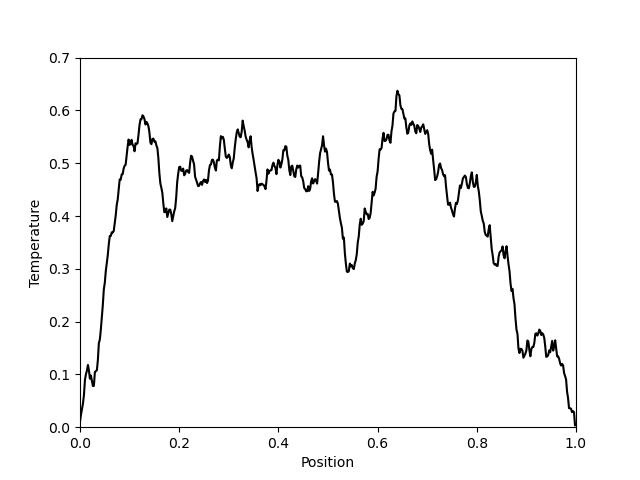
\includegraphics[width=10cm,height=6cm]{forward_heat_equation.png}
\end{figure}
\end{frame}



\begin{frame}
\frametitle{1D Heat Equation}
\begin{subequations}
  \begin{align*}
    u_t &= \Delta u &&\qquad \text{in } [0,1] \times [0,\infty),\\
      u &= 0 &&\qquad \text{on } \{0, 1\} \times [0,\infty),\\
        u &= u_0 &&\qquad \text{on }[0,1] \times \{0\}.
  \end{align*}
\end{subequations}


\begin{figure}
  \centering
  \href{run:forward_heat_equation.mp4}{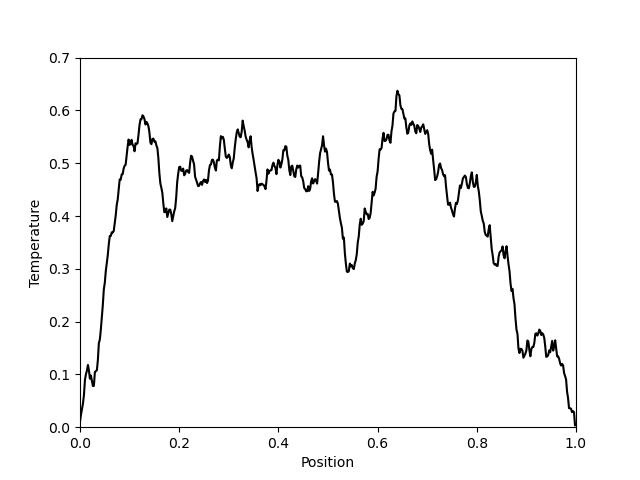
\includegraphics[width=10cm,height=6cm]{forward_heat_equation.png}}    

  %% \includemovie[inline=false,text={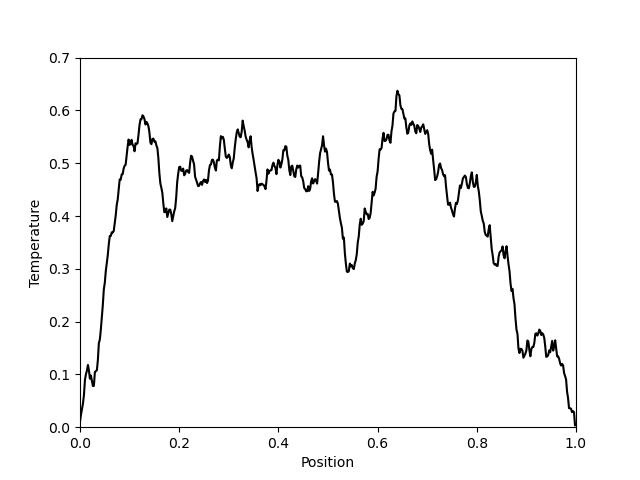
\includegraphics[scale=0.25]{forward_heat_equation.png}}]{}{}{forward_heat_equation.mp4}
  %% \flashmovie[width=12cm,height=8cm,engine=flv-player,auto=1]{forward_heat_equation.mp4}
  %% \movie[width=10cm,height=6cm,poster,autostart,loop]{
  %%   %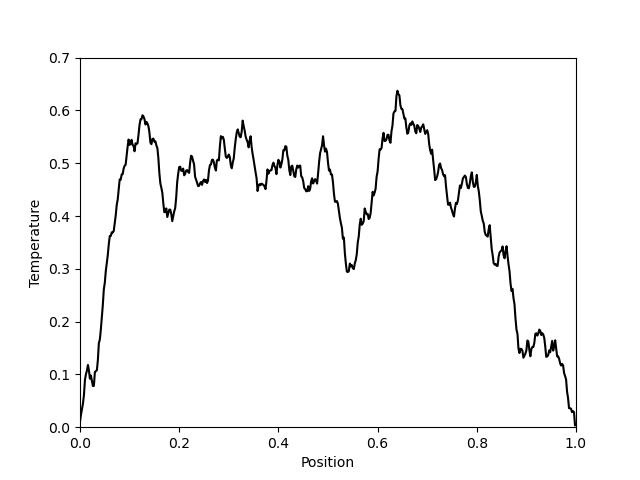
\includegraphics[width=10cm,height=6cm]{forward_heat_equation.png}
  %% }{forward_heat_equation.mp4}
\end{figure}
\end{frame}


\begin{frame}
\frametitle{Inverse Problems}
% Explain the inverse problems for the ball toss, flow field examples
% Argue that there are many valid solutions
% Explain that such problems are ill-posed

\begin{itemize}
  \item<1-> \(\fwd: \hil \to \hil\). 
  \item<2-> \(\obs u = (\meas_1^*u, \dots, \meas_m^*u )^t \in \R^m\).
  \item<3-> \(\data := \obs \fwd \param + \eps \text{ where } \eps \sim \mathcal{N}(0,\sigma^2 I_m)\)
\end{itemize}

% Show "sensor" and discuss measurement placement

% Present the entire formalism of inverse problems from the paper, for zero model error
\end{frame}


\begin{frame}
  \frametitle{Ill Posedness}
  %% \begin{figure}
    \href{run:reversed_heat_equation.mp4}{\includegraphics[width=10cm,height=6cm]{reversed_heat_equation.png}}    
  %%   \movie[width=10cm,height=6cm,poster,autostart,loop]{
  %%     \includegraphics[width=10cm,height=6cm]{reversed_heat_equation.png}
  %% }{reversed_heat_equation.mp4}
  %% \end{figure}
\end{frame}


\begin{frame}
\frametitle{Bayesian Inverse Problems (Stuart 2010)}
\begin{itemize}
\item \(\fwd: \hil \to \hil\). 
\item \(\obs u = (\meas_1^*u, \dots, \meas_m^*u )^t \in \R^m\).
\item \(\data := \obs \fwd \param + \eps \text{ where } \eps \sim \mathcal{N}(0,I_m)\)
\item \(\pr \sim \mathcal{N}(\prmean, \prcov)\).
\item \(\post \sim \mathcal{N}(\postmean, \postcov)\).
\end{itemize}

% Introduce prior and posterior measurea 
\end{frame}

\begin{frame}
\frametitle{Gaussian measures on Hilbert spaces}
\begin{figure}
   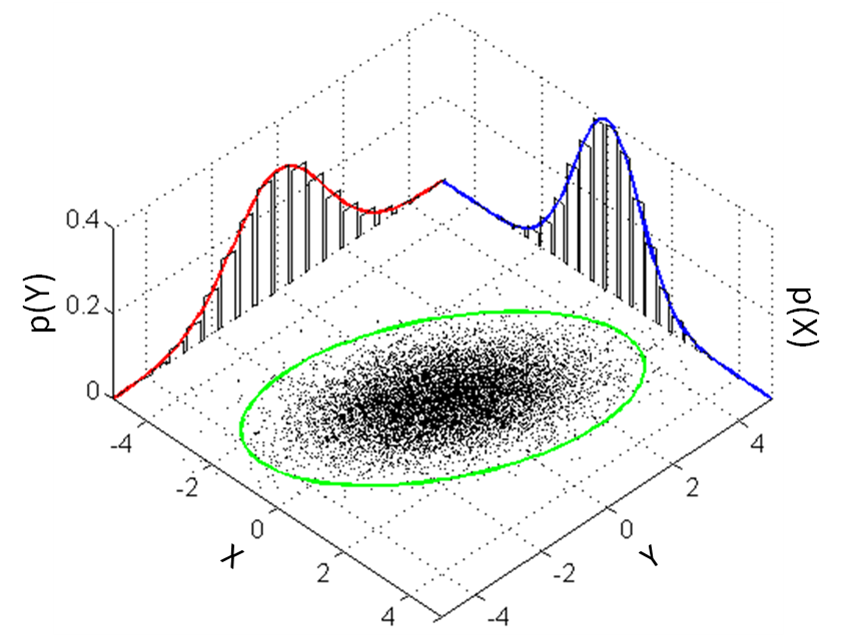
\includegraphics[width=10cm,height=6cm]{MultivariateNormal.png}
\end{figure}

\begin{align*}
  \postcov^{-1} = \prcov^{-1} + \fwd^* \obs^*\obs \fwd
\end{align*}

% Define Gaussian measure
% Show a 2D example with iso-density lines and projections
% Introduce notation for mean $\mathbf{m}$ and covariance $\Gamma$
\end{frame}

% Slide 8: Recap and notation summary
\begin{frame}
\frametitle{Recap and notation summary}

\begin{itemize}
\item Hilbert space \(\hil\) 
\item Forward operator \(\fwd: \hil \to \hil\).
%\item Observation operator \(\obs: \hil \to \mathbb{R}^m\).
\item Observation operator \(\obs u = (\meas_1^*u, \dots, \meas_m^*u )^t \in \R^m,\ u \in \hil\).
\item Data \(\data := \obs \fwd \param + \eps,\ \eps \sim \mathcal{N}(0,I_m)\).
\item Prior \(\pr\) with covariance \(\prcov\).
\item Posterior \(\post\) with covariance \(\postcov^{-1} = \prcov^{-1} + \fwd^* \obs^*\obs \fwd\)
\end{itemize}
%% 1D heat equation
\end{frame}

\begin{frame}
  Best \(\obs\) maximizes \(D_{\text{KL}} (\post || \pr )\).
\end{frame}

% Slide 10: D-optimality criterion
\begin{frame}
  \frametitle{D-optimality criterion}
  \begin{theorem}[Alexanderian, Gloor, Ghattas \cite{AlexanderianGloorGhattas14}]\label{thm:d optimality}
    Let \(\pr = \normal(\prmean,\prcov)\) a Gaussian prior on \(\hil\)
    and let \(\post = \normal(\postmean,\postcov)\) the posterior.
    %% measure on \(\hil\) for the Bayesian linear inverse problem
    %% \(\data = \obs \fwd\param + \eps\).
    Then
    \begin{align*}
      \begin{split}
        \tar( \obs) :&= \mathbb{E}_{\data}\left [ D_{\text{KL}} (\post || \pr ) \right ] \\
        % 
        % 
        % 
        &= \frac12 \log \det 
        ( I +  \prcov^{1/2}  \fwd ^* \obs^* \obs \fwd \prcov^{1/2}).
      \end{split}
    \end{align*}
  \end{theorem}

% Show the D-optimality criterion from Alexanderian et al.
% Assume linear forward operator and linear observation operator
\end{frame}

\begin{frame}
  \frametitle{Intuition}
  \begin{align*}
  \begin{split}
    \tar(\obs) &= \frac12 \log \det ( I + \prcov^{1/2}  \fwd ^* \obs^* \obs \fwd \prcov^{1/2})\\ 
    &= \frac12 \log \det \Big( \prcov ( \prcov^{-1} +  \fwd ^* \obs^* \obs \fwd) \Big )\\
    &= \frac12 \log \det \prcov \postcov^{-1}.
    %%  &= \frac12 \log \det \prcov -\frac12 \log \det \postcov.
  \end{split}
  \end{align*}
\end{frame}


\begin{frame}
  Recall \(\tar( \obs) = \frac12 \log \det ( I + 
  \prcov^{1/2} \fwd ^* \obs^* \obs \fwd \prcov^{1/2})\).

  \begin{definition}
  \(\obs^{\star}\) is \emph{D-optimal} if \(\obs^{\star} =
  \argmax_{\obs} \tar(\obs)\).
  \end{definition}
  
  %% , where entries of \(\obs \in (\hil^*)^m\)
  %% are constrained to some allowed set of measurements in \(\hil^*\). 

  %% \(\obs\) must be constrained somehow! E.g.~norm has to be bounded.
\end{frame}


\begin{frame}
\frametitle{Problem: Sensor clusterization}
\begin{figure}
    \centering
    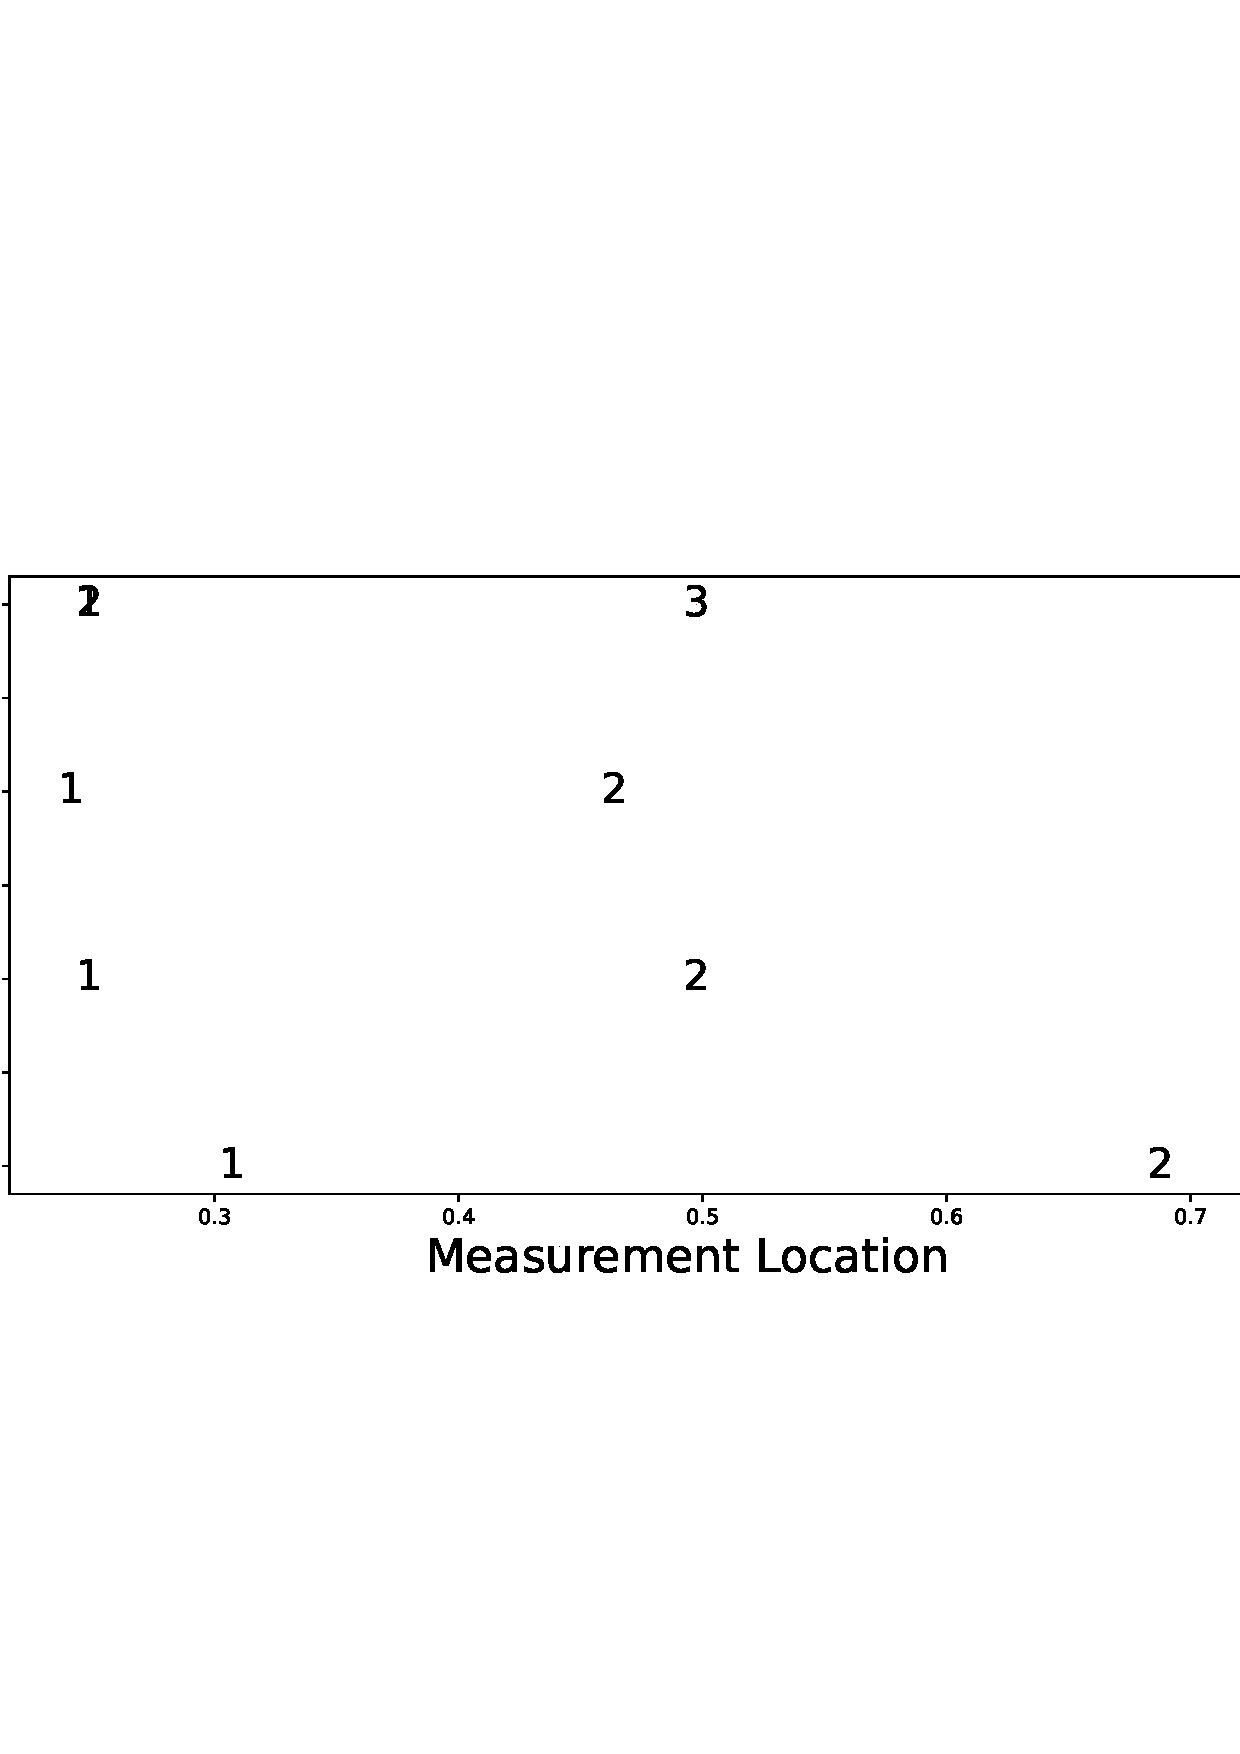
\includegraphics[height=0.5\textwidth]{example.pdf}
\end{figure}

% Discuss sensor clusterization in the 1D heat equation example
% Show figure from the paper (placeholder for figure)
\end{frame}

\begin{frame}
  \frametitle{Avoiding clusterization}

  \begin{columns}
    \begin{column}{0.6\textwidth}
      \begin{itemize}
      \item<1> Distance constraints, correlated errors (Ucinski 2005).
      \item<2> Merging close measurements (Fedorov 1997).
      \item<3> A finite set of locations (Alexanderian et al. 2020).
      \end{itemize}
    \end{column}
    \begin{column}{0.55\textwidth}
      \only<1>{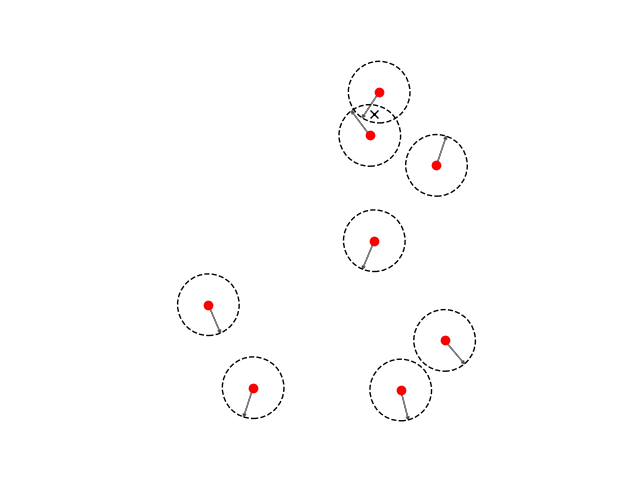
\includegraphics[width=\textwidth]{constraints.png}}
      \only<2>{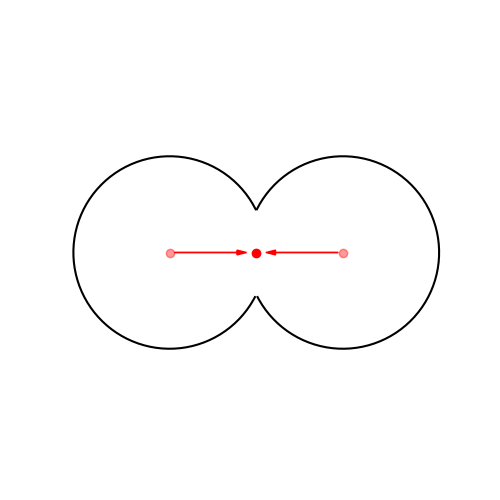
\includegraphics[width=\textwidth]{merge.png}}
      \only<3>{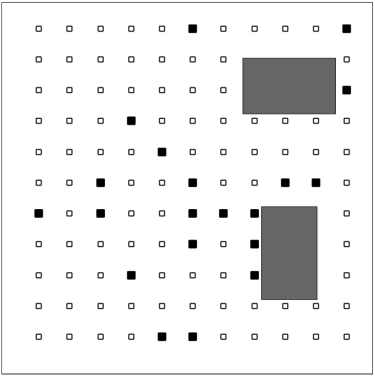
\includegraphics[width=\textwidth]{stadler_OED.png}}
    \end{column}
  \end{columns}  
\end{frame}



\begin{frame}
\frametitle{Generic Questions}
\begin{itemize}
\item Why does imposing correlations between observations alleviate
measurement clusterization?
%
\item Is measurement clusterization a generic phenomenon?
%
\item And, most importantly: Why does measurement clusterization occur?
% How do we tackle this problem?
\end{itemize}
\end{frame}

\begin{frame}
\frametitle{A "generic" inverse problem}

\begin{itemize}
\item Hilbert space \(\hil\).
\item Forward operator \(\fwd: \hil \to \hil\).
\item Observations \(\obs u = (\meas_1^*u, \dots, \meas_m^*u )^t \in \R^m,\).
\item Prior and posterior covariance \( \prcov, \postcov\).
\item Data \(\data := \obs \fwd \param + \eps\).
\item \(\tar( \obs) = \frac12 \log \det ( I + 
  \prcov^{1/2} \fwd ^* \obs^* \obs \fwd \prcov^{1/2})\).
\item \(\obs^{\star}\) is \emph{D-optimal} if \(\obs^{\star} =
  \argmax_{\obs} \tar(\obs)\).
\end{itemize}

\(\obs\) must be constrained somehow! E.g.~norm has to be bounded.
Constrain \(\meas_j\) to the unit ball \(B_{\hil} := \{x\in \hil| \|x\| = 1\}\).

%% \begin{align}\label{eq:objective}
%%   \begin{split}
%%     \tar( \obs) &= \frac12 \log \det 
%%     ( I + \prcov^{1/2}  \fwd ^* \obs^* \obs \fwd \prcov^{1/2}).
%%   \end{split}
%% \end{align}

% Discuss the main obstacle: the measurement operator
% Impose unit-norm constraints
% Explain that sensors have a unit inf-norm (show example)
% Show relevant equation from the paper
\end{frame}

% Slide 15: Constrained optimization problem
\begin{frame}
\frametitle{Constrained optimization problem}
% Restate the optimization criterion from Alexandrian et al.'s theorem
% Restate the unit norm constraints
% Pose the problem as a constrained optimization problem
% Ask the audience how to solve constrained optimization problems (Lagrange multipliers)
\begin{align*}
  \begin{split}
  \obs &= \argmax\tar(\obs)\\
  \text{subject to }& \|\meas_j\| = 1 \text{ for } j=1,\dots,m.
  \end{split}
\end{align*}

Where
\begin{align*}
  \begin{split}
    \tar(\obs) %:&= \mathbb{E}_{\data}\left [ D_{\text{KL}} (\post || \pr ) \right ] \\
    % 
    % 
    % 
    &= \frac12 \log \det ( I + \prcov^{1/2} \fwd ^* \obs^* \obs \fwd
    \prcov^{1/2}).
  \end{split}
\end{align*}
\end{frame}

\begin{frame}
%% \frametitle{Necessary conditions for optimality}
% Present the nonlinear eigenvalue problem for the vanishing model error case
% Explain why it is called a "nonlinear" eigenvalue problem

%% \begin{theorem}[Necessary conditions for D-Optimality]
  Let:
  \begin{align*}
    \begin{split}
      \obs &= \argmax\tar(\obs)\\
      \text{subject to }& \|\meas_j\| = 1 \text{ for } j=1,\dots,m.
    \end{split}
  \end{align*}
  
  Then:
  \[
   \fwd \postcov \fwd^* \obs^* = \obs^* \Xi
  \]

  %% \begin{equation*}
  %%    \fwd \postcov \fwd^* \obs^* = \obs^* \Xi, 
  %% \end{equation*}
  where \(\Xi \in \mathbb{R}^{m \times m}\) is diagonal.
%% \end{theorem}

\end{frame}


\begin{frame}
%% \frametitle{Implication of first-order conditions}
  \frametitle{Theorem (part 1)}

  \begin{gather*}
    \fwd\prcov\fwd^* \text{ and } \obs^* \obs \text{ are simultaneously diagonalizable}.\\
    \Uparrow \\
    \onslide<2->{\left( (\fwd\prcov\fwd^*)^{-1} + \obs^* \obs \right)^{-1} \obs^* = \obs^* \Xi \\
    \Uparrow  \\
    \fwd  \left(\prcov^{-1} + \fwd^* \obs^*\obs \fwd \right)^{-1} \fwd^* \obs^* = \obs^* \Xi  \\
    \Uparrow}  \\
    \fwd \postcov \fwd^* \obs^* = \obs^* \Xi  \\
  \end{gather*}
\end{frame}


\begin{frame}
  %\frametitle{Simultaneous diagonizability}
  \begin{lemma}
    %% Let \(\hil\) separable Hilbert space,
    Let \(C:\hil \to \hil\) with orthogonal eigenbasis.
    %% and \(\func_1,\dots,\func_m \in \hil\). Denote \(\func^*\) the element
    %% \(\func\) acting as a linear functional. If
  \begin{equation*}
    (C + \sum_{j=1}^m \func_j\func_j^*) \func_l = \xi_l \func_l,\ l = 1, \dots, m.
  \end{equation*}
  $\Rightarrow$ \(C\) and \(\sum_{j=1}^m \func_j \func_j^*\) are simultaneously
  diagonalizable.
  \end{lemma}
Proof idea: Consider invariant space of each eigenvalue, use spectral decomposition.
\end{frame}


\begin{frame}
  \frametitle{Theorem (part 2)}
  Let:
  \begin{itemize}
  \item \(\{\eta_i\}_{i=1}^{\infty}\) eigenvalues of \(\obs^*\obs\).
  \item \(\{\lambda_i\}_{i=1}^{\infty}\) corresponding eigenvalues of \(\fwd \prcov \fwd^*\).
  \item \(\obs\) D-optimal.
  \end{itemize}
  Then \(\eta_i > 0\) for eigenvectors corresponding to largest \(\lambda_i\).

  How many? \(\rank \obs^*\obs\).

  Why?
  \begin{align*}
    \det(I + \prcov^{1/2}  \fwd ^* \obs^* \obs \fwd \prcov^{1/2}) \sim \prod (1+\lambda_i\eta_i)
  \end{align*}
    %% INTRODUCE CYLINDERS!!!!
\end{frame}


\pgfplotstableread{
  Label     prior  optimal  sub-optimal  worst
  1         0.2    1.8           1.7      1.7
  2         0.8    1.2           0.8      0.0
  3         2.2    0             0.5      0.5
  4         3.5    0             0.0      0.0
}\optimalvsnot

\begin{frame}
  \begin{figure}
    \centering
    \begin{tikzpicture}[scale=0.6]
      \begin{axis}[
          ybar stacked,
          ymin=0,
          ymax=4,
          xtick=data,
          legend style={cells={anchor=east}, legend pos=north west, legend columns=-1},
          reverse legend=false, % set to false to get correct display, but I'd like to have this true
          xticklabels from table={\optimalvsnot}{Label},
          xticklabel style={text width=2cm,align=center},
          legend plot pos=right,
          ylabel={\LARGE precision --- prior and posterior},
          xlabel={\LARGE eigenvector},
        ]
        \addplot [fill=blue!60]  table [y=prior,   meta=Label, x expr=\coordindex] {\optimalvsnot};
        \addplot [pattern=north east lines, pattern color=green!80]  table [y=optimal, meta=Label, x expr=\coordindex] {\optimalvsnot};     
        \addlegendentry[scale=1.4]{$\lambda_i^{-1}$}
        \addlegendentry[scale=1.4]{optimal $\eta_i$s}
      \end{axis}
    \end{tikzpicture}
    \begin{tikzpicture}[scale=0.6]
      \begin{axis}[
          ybar stacked,
          ymin=0,
          ymax=4,
          xtick=data,
          legend style={cells={anchor=east}, legend pos=north west, legend columns=-1},
          reverse legend=false, % set to false to get correct display, but I'd like to have this true
          xticklabels from table={\optimalvsnot}{Label},
          xticklabel style={text width=2cm,align=center},
          legend plot pos=right,
          ylabel={\LARGE precision --- prior and posterior},
          xlabel={\LARGE eigenvector} ,
        ]   
        \addplot [fill=blue!60]  table [y=prior,       meta=Label, x expr=\coordindex] {\optimalvsnot};
        \addplot [pattern=north east lines, pattern color=green!80]  table [y=worst, meta=Label, x expr=\coordindex] {\optimalvsnot};
        \addlegendentry[scale=1.4]{$\lambda_i^{-1}$}
        \addlegendentry[scale=1.4]{sub-optimal $\eta_i$s}
      \end{axis}
    \end{tikzpicture}
  \end{figure}
\end{frame}


%% \begin{frame}
%% %% \begin{proposition}
%%   Let \(\tar: \mathbb{R}^m \to \mathbb{R}\), \(\tar(\eta) =
%%   \frac{1}{2}\sum_{i=1}^m \log (1+\lambda_i \eta_i)\), with
%%   \(\lambda_i > 0\). Then the maximum of \(\tar\)
%%   subject to \(\eta_i \geq 0\) and \(\sum\eta_i = m\) is obtained at
%%   \begin{equation}
%%   \eta_i = \begin{cases}
%%     \frac{m}{k} -  \lambda_i^{-1} +  \frac{1}{k} \sum_{j\in A} \lambda_j^{-1} & i \in A \\
%%     0 & i \in A^c
%%   \end{cases}
%%   \end{equation}
%%   where \(A:= \{1\leq i \leq m: \eta_i > 0\}\) and \(A^c = \{1,\dots, m\}
%%   \backslash A\), and \(k = |A|\), the cardinality of \(A\).
%% %% \end{proposition}
%% \end{frame}


\begin{frame}
  \frametitle{Theorem (part 3)}
  The covariance of the pushforwad \(\fwd_{*} \post\)
  %is \(\left ( (\fwd \prcov \fwd^*)^{-1} +  \obs^*\obs
  %\right )^{-1}\) and its
  has eigenvalues 
  \begin{equation*}
    \theta_i =
    \begin{cases}
      \left(\frac{\sum_{j=1}^k \lambda_j^{-1} + m}{k} \right )^{-1} & i \leq k \\
      \lambda_i &  i > k 
    \end{cases}
  \end{equation*}
\end{frame}

\begin{frame}
  \begin{figure}
    \centering
    \begin{tikzpicture}[scale=0.6]
      \begin{axis}[
          ybar stacked,
          ymin=0,
          ymax=4,
          xtick=data,
          legend style={cells={anchor=east}, legend pos=north west, legend columns=-1},
          reverse legend=false, % set to false to get correct display, but I'd like to have this true
          xticklabels from table={\optimalvsnot}{Label},
          xticklabel style={text width=2cm,align=center},
          legend plot pos=right,
          ylabel={\LARGE precision --- prior and posterior},
          xlabel={\LARGE eigenvector},
        ]
        \addplot [fill=blue!60]  table [y=prior,   meta=Label, x expr=\coordindex] {\optimalvsnot};
        \addplot [pattern=north east lines, pattern color=green!80]  table [y=optimal, meta=Label, x expr=\coordindex] {\optimalvsnot};     
        \addlegendentry[scale=1.4]{$\lambda_i^{-1}$}
        \addlegendentry[scale=1.4]{optimal $\eta_i$s}
      \end{axis}
    \end{tikzpicture}
    \begin{tikzpicture}[scale=0.6]
      \begin{axis}[
          ybar stacked,
          ymin=0,
          ymax=4,
          xtick=data,
          legend style={cells={anchor=east}, legend pos=north west, legend columns=-1},
          reverse legend=false, % set to false to get correct display, but I'd like to have this true
          xticklabels from table={\optimalvsnot}{Label},
          xticklabel style={text width=2cm,align=center},
          legend plot pos=right,
          ylabel={\LARGE precision --- prior and posterior},
          xlabel={\LARGE eigenvector} ,
        ]   
        \addplot [fill=blue!60]  table [y=prior,       meta=Label, x expr=\coordindex] {\optimalvsnot};
        \addplot [pattern=north east lines, pattern color=green!80]  table [y=sub-optimal, meta=Label, x expr=\coordindex] {\optimalvsnot};
        \addlegendentry[scale=1.4]{$\lambda_i^{-1}$}
        \addlegendentry[scale=1.4]{sub-optimal $\eta_i$s}
      \end{axis}
    \end{tikzpicture}
  \end{figure}
\end{frame}

\begin{frame}
  \frametitle{Four Sensors in the 1D Heat Equation}
  \begin{figure}
    \centering
    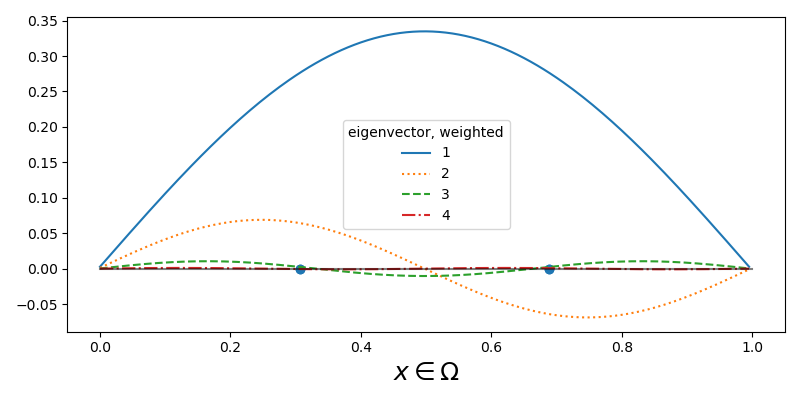
\includegraphics[width=\textwidth]{eigenvectors.pdf}
  \end{figure}
\end{frame}

\begin{frame}
  \frametitle{Summary}
  \begin{itemize}
  \item Study a generic inverse problem with unit ball constraints.
  \item D-optimality implies \(\fwd \postcov\fwd^* \obs^* = \obs^* \Xi\).
  \item Key: $\obs^*\obs$ and \(\fwd \prcov\fwd^* \obs^*\) are
    simultaneously diagonalizable.
  \item A D-optimal design concentrates on smallest prior covariance eigenvectors...
  \item ... and a D-optimal design reduces uncertainty uniformly on these.
  \item Saw manifestation in the 1D heat equation.
  \item Clusterization is just a result of avoiding higher eigenvectors
    and pigeonhole principle.
  \item Did not review: correlated errors, genericity of clusterization.
  \end{itemize}
\end{frame}
\end{document}
